\documentclass[tikz, border=10pt]{standalone}
\usetikzlibrary{mindmap}
\begin{document}
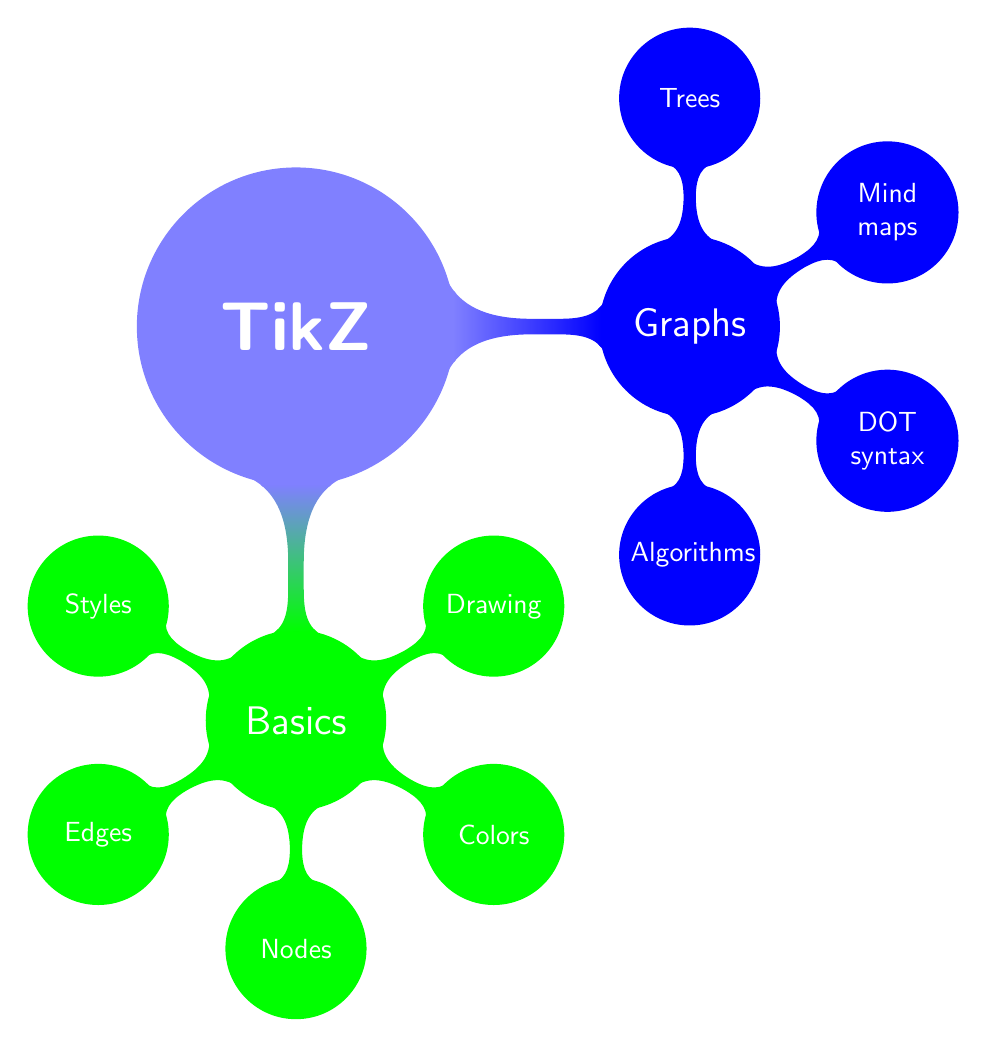
\begin{tikzpicture}[mindmap, concept color=blue!50, text=white, nodes={concept},
    root/.append style={font=\Huge\sffamily\bfseries},
    level 1 concept/.append style={
        font=\Large\sffamily, sibling angle=90
    },
    level 2 concept/.append style={
        font=\normalsize\sffamily
    }
    ]
    \node [root] {TikZ} [clockwise from=0]
        child [concept color=blue]{
            node {Graphs}[clockwise from=90]
                child {node {Trees}}
                child {node {Mind maps}}
                child {node {DOT syntax}}
                child {node {Algorithms}}
        }
        child [concept color=green] {
            node {Basics} [clockwise from=30]
                child { node {Drawing} }
                child { node {Colors} }
                child { node {Nodes} }
                child { node {Edges} }
                child { node {Styles} }
            };
\end{tikzpicture}
\end{document}